\chapter{Teorema di König ed energia cinetica}
\begin{definition}{}
Sia \(\underline{v}=\dot{\underline{x}}\) la velocità di un punto materiale di massa \(m\). Definiamo energia cinetica del punto la quantità
\[
T=m\frac{\underline{v}\cdot\underline{v}}{2}=m\frac{v^2}{2}
\]
Per un sistema di punti ciascuno di velocità \(\underline{v_i}\) e massa \(m_i\) si dice energia cinetica del sistema la quantità
\[
T=\sum_{i=1}^{n} m_i\cdot\frac{v_i^2}{2}
\]
\end{definition}
Prima di enunciare e dimostrare il teorema di König abbiamo bisogno del seguente lemma

\begin{lemma}{}
Siano \(\underline{a},\underline{b},\underline{c}\in\mathbb{R}^3\). Allora valgono le uguaglianze
\[
\underline{a}\cdot(\underline{b}\wedge\underline{c})=\underline{c}\cdot(\underline{a}\wedge\underline{b})=\underline{b}\cdot(\underline{c}\wedge\underline{a})
\]
\end{lemma}

\begin{proof}
Dimostriamo solo la prima uguaglianza perché la seconda è di nuovo la prima cambiando il ruolo dei vettori.
\begin{align*}
\underline{b}\wedge\underline{c}
&=(b_1\hat{\imath}+b_2\hat{\jmath}+b_3\hat{k})\wedge(c_1\hat{\imath}+c_2\hat{\jmath}+c_3\hat{k})
=b_1c_2\hat{k}-b_1c_3\hat{\jmath}-\hat{k}b_2c_1+b_2c_3\hat{\imath}+\\
&\quad +b_3c_1\hat{\jmath}-b_3c_2\hat{\imath}
=(b_2c_3-b_3c_2)\hat{\imath}+(b_3c_1-b_1c_3)\hat{\jmath}+(c_2b_1-c_1b_2)\hat{k}
\\[0.5em]
\underline{a}\wedge\underline{b}
&=(a_2b_3-a_3b_2)\hat{\imath}+(a_3b_1-a_1b_3)\hat{\jmath}+(b_2a_1-a_2b_1)\hat{k}
\\[0.5em]
\underline{a}\cdot(\underline{b}\wedge\underline{c})
&=
\tikz[baseline=(X.base)]{\node[inner sep=0pt,outer sep=0pt] (X) {$a_1b_2c_3$};\draw[red,line width=0.5pt] ([yshift=-1pt]X.south west)--([yshift=-1pt]X.south east);}
-
\tikz[baseline=(X.base)]{\node[inner sep=0pt,outer sep=0pt] (X) {$a_1b_3c_2$};\draw[orange!90!black,line width=0.5pt] ([yshift=-1pt]X.south west)--([yshift=-1pt]X.south east);}
+
\tikz[baseline=(X.base)]{\node[inner sep=0pt,outer sep=0pt] (X) {$a_2b_3c_1$};\draw[green!60!black,line width=0.5pt] ([yshift=-1pt]X.south west)--([yshift=-1pt]X.south east);}
-
\tikz[baseline=(X.base)]{\node[inner sep=0pt,outer sep=0pt] (X) {$a_2b_1c_3$};\draw[blue,line width=0.5pt] ([yshift=-1pt]X.south west)--([yshift=-1pt]X.south east);}
+
\tikz[baseline=(X.base)]{\node[inner sep=0pt,outer sep=0pt] (X) {$a_3c_2b_1$};\draw[violet,line width=0.5pt] ([yshift=-1pt]X.south west)--([yshift=-1pt]X.south east);}
-
\tikz[baseline=(X.base)]{\node[inner sep=0pt,outer sep=0pt] (X) {$a_3c_1b_2$};\draw[red!70!magenta,line width=0.5pt] ([yshift=-1pt]X.south west)--([yshift=-1pt]X.south east);}
\\[0.5em]
\underline{c}\cdot(\underline{a}\wedge\underline{b})
&=
\tikz[baseline=(X.base)]{\node[inner sep=0pt,outer sep=0pt] (X) {$c_1a_2b_3$};\draw[green!60!black,line width=0.5pt] ([yshift=-1pt]X.south west)--([yshift=-1pt]X.south east);}
-
\tikz[baseline=(X.base)]{\node[inner sep=0pt,outer sep=0pt] (X) {$c_1a_3b_2$};\draw[red!70!magenta,line width=0.5pt] ([yshift=-1pt]X.south west)--([yshift=-1pt]X.south east);}
+
\tikz[baseline=(X.base)]{\node[inner sep=0pt,outer sep=0pt] (X) {$c_2a_3b_1$};\draw[violet,line width=0.5pt] ([yshift=-1pt]X.south west)--([yshift=-1pt]X.south east);}
-
\tikz[baseline=(X.base)]{\node[inner sep=0pt,outer sep=0pt] (X) {$c_2a_1b_3$};\draw[orange!90!black,line width=0.5pt] ([yshift=-1pt]X.south west)--([yshift=-1pt]X.south east);}
+
\tikz[baseline=(X.base)]{\node[inner sep=0pt,outer sep=0pt] (X) {$c_3b_2a_1$};\draw[red,line width=0.5pt] ([yshift=-1pt]X.south west)--([yshift=-1pt]X.south east);}
-
\tikz[baseline=(X.base)]{\node[inner sep=0pt,outer sep=0pt] (X) {$c_3a_2b_1$};\draw[blue,line width=0.5pt] ([yshift=-1pt]X.south west)--([yshift=-1pt]X.south east);}
\end{align*}
\end{proof}

\begin{theorem}{}[di König]
L'energia cinetica di un corpo rigido è pari a
\[
T=m\frac{\underline{v_G}\cdot\underline{v_G}}{2}+\frac{1}{2}\,\underline{\omega}\cdot I_G\underline{\omega}
\]
\end{theorem}

\begin{proof}
Ricordiamo dalla lezione sulla seconda equazione cardinale che
\[
\underline{x_G}=\frac{\sum_i m_i\underline{x_i}}{\sum_i m_i}
\qquad
\underline{v_G}=\frac{\sum_i m_i\underline{v_i}}{m}
\qquad
\underline{x_i}=\underline{x_G}+\underline{x_i'}
\qquad
\sum_i m_i\underline{x_i'}=0 \Rightarrow \sum_i m_i\underline{v_i'}=0
\quad
\sum_i \underline{x_i'}\wedge m_i\underline{v_i'}=I_G\underline{\omega}
\]

\begin{align*}
2T
&=\sum_i m_i\cdot v_i^2
=\sum_i m_i\cdot(\underline{v_G}+\underline{v_i'})\cdot(\underline{v_G}+\underline{v_i'}) \\
&=\sum_i m_i\,\underline{v_G}\cdot\underline{v_G}
+2\sum_i m_i\,\underline{v_G}\cdot\underline{v_i'}
+\sum_i m_i\,\underline{v_i'}\cdot\underline{v_i'} \\
&=\underline{v_G}\cdot\underline{v_G}\sum_i m_i
+2\underline{v_G}\cdot\sum_i m_i\underline{v_i'}
+\sum_i m_i\,\underline{v_i'}\cdot\underline{v_i'} \\
&=m\,v_G^2+\sum_i m_i\,\underline{v_i'}\cdot\underline{v_i'}
\end{align*}

Dal momento che \(\sum_i m_i\underline{v_i'}=0 \Rightarrow 2\underline{v_G}\cdot\sum_i m_i\underline{v_i'}=0\)

Applichiamo la legge fondamentale nel sistema di riferimento del centro di massa rispetto al centro di massa : \(\underline{v_i'}=\underline{\omega}\wedge\underline{x_i'}\)

\begin{align*}
\sum_i m_i\,\underline{v_i'}\cdot\underline{v_i'}
&=\sum_i m_i\,\underline{v_i'}\cdot(\underline{\omega}\wedge\underline{x_i'}) \\
&=\sum_i m_i\,\underline{x_i'}\cdot(\underline{v_i'}\wedge\underline{\omega}) \\
&=\sum_i \underline{\omega}\cdot(\underline{x_i'}\wedge m_i\underline{v_i'}) \\
&=\underline{\omega}\cdot\left(\sum_i \underline{x_i'}\wedge m_i\underline{v_i'}\right)
=\underline{\omega}\cdot I_G\underline{\omega}
\end{align*}

Concludiamo che
\[
T=\frac{1}{2}mv_G^2+\frac{1}{2}\underline{\omega}\cdot I_G\underline{\omega}
\]
\end{proof}

\section{Energia cinetica: esempi nel piano}
Nel caso di un moto piano come abbiamo già detto \(\underline{\omega}=\omega\hat{k}\). Allora il teorema di König in un sistema di riferimento orientato secondo gli assi principali di inerzia (base di autovettori) diventa
\[
T=\frac{1}{2}mV_G^2+\frac{1}{2}I^{zz}\omega^2
\]
\begin{example}{}
Consideriamo un disco omogeneo di centro fissato massa \(m\) e raggio \(R\).

\begin{center}
\centering
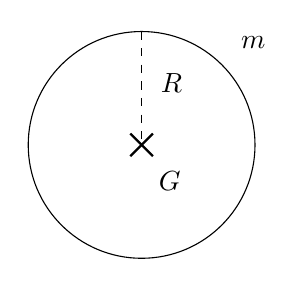
\begin{tikzpicture}[scale=1.2]
\draw (0,0) circle (1.2);
\draw[dashed] (0,1.2) -- (0,0);
\draw[thick] (-0.12,0.12) -- (0.12,-0.12);
\draw[thick] (-0.12,-0.12) -- (0.12,0.12);
\node[right] at (0.08,-0.38) {\(G\)};
\node[right] at (0.1,0.65) {\(R\)};
\node[right] at (0.95,1.08) {\(m\)};
\end{tikzpicture}
\end{center}

Sappiamo che \(I_G^{zz}=I_G=\frac{1}{2}mR^2\) e \(v_G=0\). Allora
\[
T=\frac{1}{2}\omega^2\cdot\frac{1}{2}mR^2=\frac{1}{4}mR^2\omega^2
\]
\end{example}


\begin{example}{}
Troviamo l'energia cinetica di un'asta con centro di massa fisso, lunghezza \(\ell\) e massa \(m\)

\begin{center}
\begin{tikzpicture}[scale=1.2,>=latex]
\draw[line width=0.8pt] (-1.2,-1.0) -- (1.2,1.0);

\fill (0,0) circle (2.2pt);
\draw[line width=0.8pt] (-0.12,0.12) -- (0.12,-0.12);
\draw[line width=0.8pt] (-0.12,-0.12) -- (0.12,0.12);

\node[left] at (-0.1,0.25) {\(G\)};
\node[right] at (1.02,1.18) {\(m\)};
\node[right] at (0.28,-0.52) {\(\ell\)};
\end{tikzpicture}
\end{center}

\[
I_G=\frac{m\ell^2}{12},\ v_G=0 \ \Rightarrow\ T=\frac{1}{2}\frac{m\ell^2}{12}\omega^2=\frac{m\ell^2\omega^2}{24}
\]
\end{example}
\begin{example}{}
Consideriamo ora un'asta di massa \(m\) e lunghezza \(\ell\) con un estremo fissato.

\begin{center}
\begin{tikzpicture}[scale=1.2,>=latex]
\coordinate (A) at (0,0);
\coordinate (B) at (2.6,-2.5);
\coordinate (C) at ($(A)!0.5!(B)$);

\draw[line width=0.8pt] (A) -- (B);
\draw[line width=0.8pt] (-0.08,0.18) -- (0.18,-0.08);
\draw[line width=0.8pt] (2.42,-2.32) -- (2.68,-2.58);

\draw[dashed] (A) -- (0,-2.7);

\draw[red,->] (A) -- (0.85,0);
\draw[red,->] (A) -- (0,0.95);

\node[red,right] at (0.7,0.02) {\(\hat{\imath}\)};
\node[red,left] at (0.05,0.88) {\(\hat{\jmath}\)};

\draw[thick] (A) circle (0.1);
\draw[thick] (-0.07,-0.07) -- (0.07,0.07);
\draw[thick] (-0.07,0.07) -- (0.07,-0.07);

\fill (C) circle (2pt);

\draw[->] (-0.05,-0.45) arc[start angle=-95,end angle=-50,radius=0.45];
\node[left] at (0.18,-0.92) {\(\theta\)};

\node[left] at (-0.15,0.02) {\(A\)};
\node[left] at ($(C)+(-0.08,0.15)$) {\(G\)};
\node[right] at (2.35,-2.75) {\(m\)};
\node[right] at (1.7,-1.05) {\(\ell\)};
\end{tikzpicture}
\end{center}

\[
x_G=\frac{\ell}{2}\sin\theta \qquad y_G=-\frac{\ell}{2}\cos\theta \qquad \Rightarrow \qquad \dot{x}_G=\dot{\theta}\frac{\ell}{2}\cos\theta \qquad \dot{y}_G=\dot{\theta}\frac{\ell}{2}\sin\theta
\]

Notiamo che
\[
v_G^2=\dot{x}_G^2+\dot{y}_G^2=\frac{\ell^2}{4}\dot{\theta}^2
\]
Allora
\[
T=\frac{m\ell^2\dot{\theta}^2}{8}+\frac{m\ell^2\dot{\theta}^2}{24}=\frac{m\ell^2\dot{\theta}^2}{6}=\frac{m\ell^2\omega^2}{6}
\]

Alternativamente potevamo lavorare con il teorema di Huygens e scrivere
\[
T=\frac{1}{2}I_A\omega^2=\frac{1}{2}\left(I_G+m\frac{\ell^2}{4}\right)\omega^2=\frac{1}{2}\left(\frac{m\ell^2}{12}+\frac{m\ell^2}{4}\right)\omega^2=\frac{m\ell^2}{6}\omega^2
\]
\end{example}
\begin{oss}{}
    L'uso dei momenti d'inerzia non rispetto ad un asse passante per il centro di massa per il calcolo dell'energia cinetica non l'abbiamo dimostrato in questo corso ma lo abbiamo fatto in Fisica 1 quindi lo diamo per buono!
\end{oss}

\begin{example}{}
Studiamo un disco di massa \(m\) e raggio \(r\) che rotola su una guida.

\begin{center}
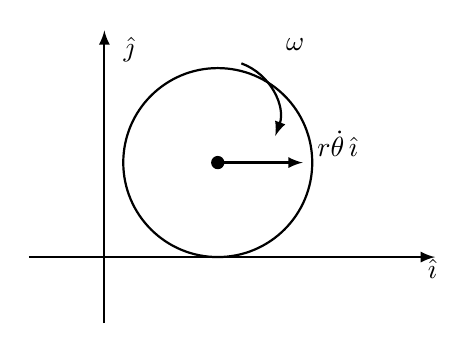
\begin{tikzpicture}[scale=1.2,>=latex]
\draw[->,line width=0.8pt] (-2,0) -- (2.3,0);
\draw[->,line width=0.8pt] (-1.2,-0.7) -- (-1.2,2.4);

\draw[line width=0.8pt] (0,1) circle (1);

\fill (0,1) circle (2pt);
\draw[->,line width=0.8pt] (0,1) -- (0.9,1);

\draw[->,line width=0.8pt] (0.25,2.05) arc[start angle=70,end angle=-20,radius=0.6];

\node[right] at (2.12,-0.12) {\(\hat{\imath}\)};
\node[right] at (-1.1,2.2) {\(\hat{\jmath}\)};
\node[right] at (0.95,1.2) {\(r\dot{\theta}\,\hat{\imath}\)};
\node[right] at (0.62,2.25) {\(\omega\)};
\end{tikzpicture}
\end{center}

Dal moto di puro rotolamento sappiamo che \(\underline{v_G}=r\dot{\theta}\,\hat{\imath}\)

\[
T=\frac{1}{2}m(r\dot{\theta})^2+\frac{1}{2}\left(\frac{1}{2}mr^2\right)\dot{\theta}^2=\frac{1}{2}mr^2\dot{\theta}^2+\frac{1}{4}mr^2\dot{\theta}^2=\frac{3}{4}mr^2\dot{\theta}^2
\]
\end{example}

\begin{example}{}
Studiamo il moto di un disco di massa \(M\) e raggio \(R\) che rotola su un piano orizzontale. Avvolto attorno al disco c'è un filo inestensibile teso e fatto passare attorno ad un piolo di altezza \(2R\). All'altra estremità del disco è appesa una massa \(m\). All'istante \(t=0\) lasciamo cadere la massa con velocità nulla e filo verticale dalla posizione del piolo.


\begin{center}
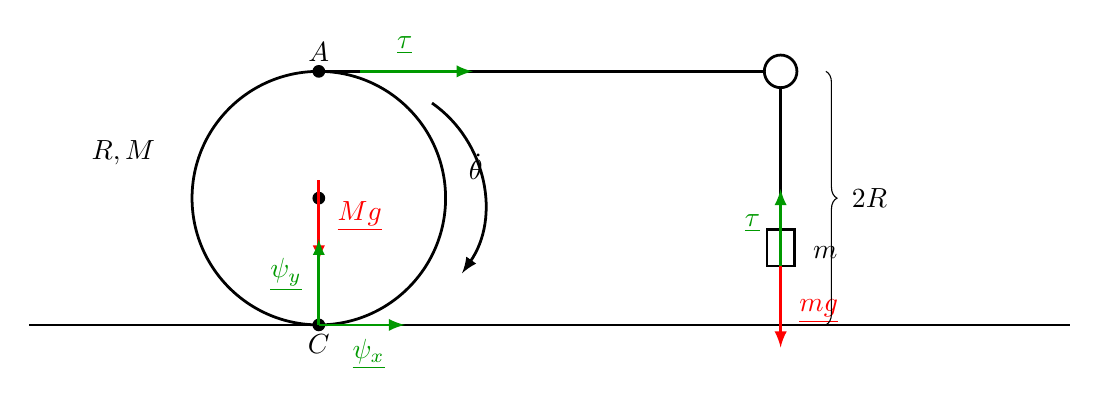
\begin{tikzpicture}[scale=1.15,>=latex]

% parametri
\def\R{1.4}

% piano
\draw[line width=1pt] (-3.2,0) -- (8.3,0);

% disco
\draw[line width=1pt] (0,\R) circle (\R);
\fill (0,\R) circle (2pt);

% punti A e C
\fill (0,2*\R) circle (2pt);
\fill (0,0) circle (2pt);
\node[above] at (0,2*\R) {\(A\)};
\node[below] at (0,0) {\(C\)};

% etichetta R,M
\node[left] at (-1.7,1.9) {\(R,M\)};

% peso disco
\draw[red,->,line width=1pt] (0,\R+0.2) -- (0,\R-0.7);
\node[red,right] at (0.1,\R-0.2) {\(\underline{Mg}\)};

% reazioni al contatto
\draw[green!60!black,->,line width=1pt] (0,0) -- (0.95,0);
\node[green!60!black,below] at (0.55,-0.05) {\(\underline{\psi_x}\)};

\draw[green!60!black,->,line width=1pt] (0,0) -- (0,0.95);
\node[green!60!black,left] at (-0.08,0.55) {\(\underline{\psi_y}\)};

% filo orizzontale e piolo
\draw[line width=1pt] (0,2*\R) -- (4.9,2*\R);
\draw[line width=1pt] (5.1,2*\R) circle (0.18);
\draw[line width=1pt] (5.1,2*\R-0.18) -- (5.1,1.05);

% massa appesa
\draw[line width=1pt] (4.95,1.05) rectangle (5.25,0.65);
\node[right] at (5.35,0.8) {\(m\)};

% tensioni
\draw[green!60!black,->,line width=1pt] (0.45,2*\R) -- (1.7,2*\R);
\node[green!60!black,above] at (0.95,2*\R+0.08) {\(\underline{\tau}\)};

\draw[green!60!black,->,line width=1pt] (5.1,0.65) -- (5.1,1.5);
\node[green!60!black,left] at (4.98,1.12) {\(\underline{\tau}\)};

% peso massa
\draw[red,->,line width=1pt] (5.1,0.65) -- (5.1,-0.25);
\node[red,right] at (5.2,0.15) {\(\underline{mg}\)};

% freccia di rotazione esterna al disco
\draw[->,line width=1pt] (1.25,2.45) arc[start angle=55,end angle=-35,radius=1.35];
\node[right] at (1.55,1.75) {\(\dot{\theta}\)};

% quota 2R
\draw[decorate,decoration={brace,amplitude=4pt}] (5.6,2*\R) -- (5.6,0);
\node[right] at (5.78,\R) {\(2R\)};

\end{tikzpicture}
\end{center}


Il sistema ha un grado di libertà: il puro rotolamento lascia un grado di libertà al disco e la massa è sottoposta ai vincoli
\[
\underline{x_m}=\underline{x_{\text{ext}}^{\text{asta}}}
\]

Vogliamo legare \(y_m\) con \(\theta\).

\[
\underline{v_A}=\underline{v_C}+\underline{\omega}\wedge(\underline{x_A}-\underline{x_C})=2R\dot{\theta}\,\hat{\imath}
\]

Per il vincolo di puro rotolamento tra disco e corda si ha che
\[
\underline{v_A}\cdot\hat{t}=\underline{v_A}^{\text{disco}}\cdot\hat{t}=\underline{v_A}^{\text{filo}}\cdot\hat{t}
\]

Inoltre dal momento che \(\hat{t}\parallel \underline{v_A}\) possiamo scrivere
\[
\dot{y}_m=-2R\dot{\theta}\Rightarrow y_m=-2R\theta
\]

Calcoliamo l'energia cinetica del sistema. Usando Huygens sappiamo che
\[
I_C=\frac{MR^2}{2}+MR^2=\frac{3}{2}MR^2 \Rightarrow T_s=\frac{3}{2}MR^2\frac{\dot{\theta}^2}{2}+\frac{m\dot{y}_m^2}{2}=\frac{3}{2}MR^2\frac{\dot{\theta}^2}{2}+\frac{m4R^2\dot{\theta}^2}{2}=R^2\dot{\theta}^2\left(\frac{3}{4}M+2m\right)
\]

Vogliamo infine trovare un'espressione analitica per \(\theta(t)\). Usiamo la prima legge cardinale su \(m\) e la seconda sul disco rispetto a \(C\) come polo.

\[
\left\{
\begin{aligned}
m\ddot{y}_m&=\tau-mg\\
\frac{d}{dt}(I_C\dot{\theta})&=2R\tau
\end{aligned}
\right.
\Rightarrow
\left\{
\begin{aligned}
-2mR\ddot{\theta}&=\tau-mg\\
\frac{3}{2}MR^2\ddot{\theta}&=2R\tau
\end{aligned}
\right.
\Rightarrow
\left\{
\begin{aligned}
-2mR\ddot{\theta}&=\frac{3}{4}MR\ddot{\theta}-mg\\
\tau&=\frac{3}{4}MR\ddot{\theta}
\end{aligned}
\right.
\]

\[
\Rightarrow \left(2mR+\frac{3}{4}MR\right)\ddot{\theta}=mg \Rightarrow \ddot{\theta}=\frac{mg}{2mR+\frac{3}{4}MR}
\]

\[
\theta(0)=0
\qquad
\dot{\theta}(0)=0
\]

\[
\Rightarrow \theta(t)=\frac{mg}{2mR+\frac{3}{4}MR}\frac{t^2}{2}
\]
\end{example}

\begin{example}{}
Studiamo una variazione dell'esercizio precedente: fissiamo il piolo ad altezza \(R\). Questa volta impongo le condizioni iniziali \(\theta(0)=1\) \(x_G(0)=R\) e fisso la rotazione positiva in senso antiorario.

\begin{center}
\begin{center}
\begin{tikzpicture}[scale=1.15,>=latex]

% parametri
\def\R{2}
\def\rp{0.18}

% punti principali
\coordinate (G) at (0,\R);
\coordinate (C) at (0,0);
\coordinate (A) at ({\R*cos(70)},{\R+\R*sin(70)});
\coordinate (P) at (5.84,\R);
\coordinate (B) at ($(P)+({\rp*cos(160)},{\rp*sin(160)})$);
\coordinate (O) at (4.65,0);

% piano
\draw[line width=0.9pt] (-4,0) -- (7.2,0);

% disco
\draw[line width=0.9pt] (G) circle (\R);

% punti
\fill (G) circle (2.3pt);
\fill (C) circle (2.3pt);
\fill (A) circle (2.3pt);

% etichette punti
\node[right] at ($(G)+(0.18,0.02)$) {\(G\)};
\node[below] at ($(C)+(0,-0.03)$) {\(C\)};
\node[above right] at ($(A)+(0.18,0.18)$) {\(A\)};

% raggio GA
\draw[line width=0.9pt] (G) -- (A);
\node[left] at ($(G)!0.55!(A)+(-0.08,0.08)$) {\(R\)};

% filo inclinato
\draw[line width=0.9pt] (A) -- (B);

% piolo
\draw[line width=0.9pt] (P) circle (\rp);

% filo verticale
\draw[line width=0.9pt] ($(P)+(0,-\rp)$) -- ($(P)+(0,-2.35)$);

% massa
\draw[line width=0.9pt] ($(P)+(-0.12,-2.65)$) rectangle ($(P)+(0.12,-2.35)$);
\node[right] at ($(P)+(0.32,-2.5)$) {\(m\)};

% linea tratteggiata orizzontale
\draw[dashed,line width=0.8pt] (G) -- (P);
\node[below] at ($(G)!0.55!(P)+(0,-0.18)$) {\(R\theta\)};

% angolo alpha
\draw[line width=0.8pt] ($(P)+(-0.55,0)$) arc[start angle=180,end angle=160,radius=0.55];
\node[above left] at ($(P)+(-0.7,0)$) {\(\alpha\)};

% squadra di ortogonalità in A
\draw[line width=0.8pt]
($(A)+(-0.08,-0.17)$) --
($(A)+(0.10,-0.24)$) --
($(A)+(0.17,-0.06)$);

% versore tangente
\draw[red,->,line width=1pt] (A) -- ++(-1.05,0.38);
\node[red,above] at ($(A)+(-0.62,0.48)$) {\(\hat{t}\)};

% freccia di theta
\draw[->,line width=1pt] (-2.35,3.95) arc[start angle=125,end angle=200,radius=1.15];
\node[left] at (-2.1,3.1) {\(\theta\)};

% velocità del centro
\draw[orange!85!black,->,line width=1pt] (G) -- ++(-1.45,0);
\node[orange!85!black,above] at ($(G)+(-0.78,0.14)$) {\(R\dot{\theta}\hat{\imath}\)};

% assi locali
\draw[green!60!black,->,line width=1pt] (O) -- ++(-0.95,0);
\draw[green!60!black,->,line width=1pt] (O) -- ++(0,0.95);
\node[green!60!black,below left] at ($(O)+(0.02,-0.02)$) {\(O\)};
\node[green!60!black,left] at ($(O)+(-0.58,-0.05)$) {\(\hat{\imath}\)};
\node[green!60!black,right] at ($(O)+(0.05,0.62)$) {\(\hat{\jmath}\)};

% quota R
\draw[decorate,decoration={brace,amplitude=4pt}] ($(P)+(0.45,0)$) -- ($(P)+(0.45,-\R)$);
\node[right] at ($(P)+(0.63,-1)$) {\(R\)};

\end{tikzpicture}
\end{center}
\end{center}

\[
R=R\theta\sin\alpha \Rightarrow \theta\sin\alpha=1 \Rightarrow \sin\alpha=\frac{1}{\theta} \Rightarrow \cos\alpha=\sqrt{1-\frac{1}{\theta^2}}=\sqrt{\frac{\theta^2-1}{\theta^2}} \qquad \text{con } |\theta|\geq 1
\]

Come prima \(\underline{v_A}=\underline{v_A}^{\text{disco}}=\underline{v_A}^{\text{filo}}\)

\[
\underline{v_G}=\omega\wedge(\underline{x_G}-\underline{x_C})=R\dot{\theta}\hat{\imath}
\]

\[
\underline{v_A}=\underline{v_G}+\omega\wedge(\underline{x_A}-\underline{x_G})=R\dot{\theta}\hat{\imath}+R\dot{\theta}\hat{t}
\]

Per sapere la velocità di \(m\) devo usare solo la componente lungo \(\hat{t}\)

\[
\Rightarrow \dot{y}_m=\underline{v_A}\cdot\hat{t}=R\dot{\theta}\hat{\imath}\cdot\hat{t}+R\dot{\theta}=R\dot{\theta}\left(1+\frac{\sqrt{\theta^2-1}}{\theta}\right)
\]

L'energia cinetica del sistema è

\[
T=\frac{3}{2}MR^2\frac{\dot{\theta}^2}{2}+\frac{m}{2}R^2\dot{\theta}^2\left(1+\frac{\sqrt{\theta^2-1}}{\theta}\right)^2
\]

Dalle equazioni cardinali si può ricavare \(\theta(t)\)

\[
\left\{
\begin{aligned}
M\ddot{x}_G&=\psi_x+\tau\cos\alpha\\
M\ddot{y}_G&=\psi_y-Mg+\tau\sin\alpha\\
m\ddot{y}_m&=mg+\tau\\
\frac{MR^2}{2}\ddot{\theta}&=-\psi_xR+\tau R
\end{aligned}
\right.
\]
\end{example}
